% Provenance (never printed): see sources/outline_sources.md (Year 2: the Himalaya and Tibet;
% the Andes; crustal thickening and plateaus). Himalayan units, thrusts and rates after Lave
% and Avouac (2000), Ader et al. (2012), Cattin et al. (2001), Dong et al. (2026, STDS);
% Asian extrusion after Jiao et al. (2023); Tibetan rifts after Wang et al. (2021); Central
% Andes after Gerbault et al. (2005); flat slabs after Gauthier et al. (2024). Relief from
% ETOPO1 (figdata/bachelor-2/plateaus.py); plate velocities from NNR-MORVEL56 (Book 2 ledger
% row nnr56:poles). Exercise and problem values in the Book 4 scratch calculator
% calc/ch14.py.
\chapter{Cordilleras de colisión y cordilleras andinas comparadas}\label{ch:b2:himalaya-andes}

Dos mesetas de la Tierra se alzan a más de cuatro kilómetros de altura a lo largo de cientos de kilómetros.
El Tíbet se elevó donde la India chocó con Asia, dos continentes que se encontraron después de que desapareciera el océano que
los separaba. El Altiplano se elevó donde una placa oceánica, la placa de Nazca, sigue deslizándose
bajo Sudamérica, sin que llegue continente alguno. Dos motores distintos construyeron dos
relieves semejantes. Este capítulo desmonta las dos cordilleras, mide cuánto se ha engrosado su corteza
y por qué, y se pregunta qué les impide crecer más.
% ledger: lave00:setting, gerbault05:andes, data:b4-etopo-tibet, data:b4-etopo-andes

\begin{recall}
\textbf{Del volumen de bachillerato}: la colisión continental y la sutura; la deriva de la India
hacia el norte, su frenado y la edad discutida de la colisión; la meseta del Tíbet, de unos
\qty{4600}{m} de altura sobre una corteza de unos \qty{70}{km} de espesor. \textbf{Del volumen de primer año}:
la isostasia de Airy y la placa de Bouguer; los márgenes activos, la placa que subduce, el arco volcánico y
el espacio arco--fosa; las velocidades de placa a partir de las velocidades angulares; la ley de Byerlee; la magnitud
de momento. \textbf{Del \cref{ch:b2:crustal-melting}}: los \omterm{def:b2:crustal-melting:leucogranite}{leucogranitos} del Himalaya.
\textbf{Del \cref{ch:b2:alpine-orogen}}: el \omterm{def:b2:alpine-orogen:orogen}{orógeno}, el \omterm{def:b2:alpine-orogen:nappes}{manto de corrimiento}, el \omterm{def:b2:alpine-orogen:decollement}{despegue}, la \omterm{def:b2:alpine-orogen:skin}{tectónica de piel fina} y
de piel gruesa, el \omterm{def:b2:alpine-orogen:ftb}{cinturón de pliegues y cabalgamientos}, la \omterm{def:b2:alpine-orogen:foreland}{cuenca de antepaís}, los \omterm{def:b2:alpine-orogen:balanced}{cortes compensados}.
\end{recall}

\begin{definition}[Orógeno de colisión; orógeno de tipo andino]\label{def:b2:himalaya-andes:types}
Un \emph{orógeno de colisión}\index{orógeno de colisión} es un \omterm{def:b2:alpine-orogen:orogen}{orógeno} construido por la convergencia de
dos márgenes continentales después de que se haya consumido el océano que los separaba; su eje es una sutura.
Un \emph{orógeno de tipo andino}\index{orógeno de tipo andino} es un \omterm{def:b2:alpine-orogen:orogen}{orógeno} construido sobre la placa
cabalgante de una zona de subducción océano--continente, mientras la subducción continúa bajo él; su eje
es un arco volcánico.
\end{definition}


\section{La India contra Asia}\label{sec:b2:himalaya-andes:himalaya}

La India alcanzó el borde meridional de Eurasia hace unos 50 millones de años a lo largo de la sutura del Indo--Tsangpo,
también llamada sutura del Indo--Yarlung; la fecha exacta sigue discutiéndose, como mostró el
volumen de bachillerato. La convergencia no se detuvo. Hoy la India y Asia se acercan
a unos \qty{40}{mm} al año; según las velocidades angulares del modelo de placas NNR-MORVEL56,
la India se mueve a \qty{45}{mm} al año respecto de Eurasia en \ang{28}~N, \ang{85}~E, hacia
\ang{22} al este del norte. Solo una parte de ese movimiento se absorbe en el Himalaya. A través de Nepal,
las estaciones GPS muestran que la India y el sur del Tíbet convergen a $17.8 \pm \qty{0.5}{mm}$ al año en el
centro y el este y a $20.5 \pm \qty{1}{mm}$ al año en el oeste: cerca de la mitad del total. El resto
se reparte por el Tíbet y el resto de Asia.
% ledger: lave00:setting, najman21:collision-age, jiao23:extrusion, nnr56:poles, ader12:rates, ader12:mht
% values (plateaus.py): v_india_eurasia 44.99 mm/yr, azimuth 21.65

Los mapas siguientes muestran las dos cordilleras con las mismas curvas de nivel, y las franjas a lo largo de las cuales este
capítulo las corta.

\begin{omfigure}
\centering
% ledger: data:b4-etopo-tibet, data:b4-etopo-andes
\begin{tikzpicture}
\begin{axis}[name=tib, scale only axis, width=8.0cm, height=4.8cm, xmin=75, xmax=100,
  ymin=25, ymax=40, xlabel={longitud (\unit{\degree} E)}, ylabel={latitud (\unit{\degree} N)},
  tick label style={font=\scriptsize}, label style={font=\small}, xtick={75,80,...,100},
  ytick={25,30,...,40}, title={\small Himalaya y Tíbet}]
\addplot[omThm!35, line width=0.3pt] table[x=lon, y=lat] {figdata/out/bachelor-2-plateaus-tc2000.dat};
\addplot[omThm!90!black, line width=0.4pt] table[x=lon, y=lat] {figdata/out/bachelor-2-plateaus-tc4000.dat};
\draw[black, densely dashed, line width=0.9pt] (axis cs:86,25) rectangle (axis cs:90,40);
\node[font=\scriptsize, fill=white, fill opacity=0.85, text opacity=1, inner sep=1pt] at (axis cs:80,26.2) {llanura del Ganges};
\node[font=\scriptsize, fill=white, fill opacity=0.85, text opacity=1, inner sep=1pt] at (axis cs:94.5,33.5) {meseta del Tíbet};
\node[font=\scriptsize, fill=white, fill opacity=0.85, text opacity=1, inner sep=1pt] at (axis cs:83,39.2) {Tarim};
\end{axis}
\begin{axis}[at={(tib.east)}, anchor=west, xshift=1.6cm, scale only axis, width=3.6cm,
  height=4.8cm, xmin=-75, xmax=-60, ymin=-30, ymax=-10,
  xlabel={longitud (\unit{\degree})}, tick label style={font=\scriptsize},
  label style={font=\small}, xtick={-75,-70,-65,-60}, ytick={-30,-25,...,-10},
  title={\small Andes Centrales}]
\addplot[blue!60!black, line width=0.45pt] table[x=lon, y=lat] {figdata/out/bachelor-2-plateaus-ac0.dat};
\addplot[omThm!35, line width=0.3pt] table[x=lon, y=lat] {figdata/out/bachelor-2-plateaus-ac2000.dat};
\addplot[omThm!90!black, line width=0.4pt] table[x=lon, y=lat] {figdata/out/bachelor-2-plateaus-ac4000.dat};
\draw[black, densely dashed, line width=0.9pt] (axis cs:-75,-21) rectangle (axis cs:-60,-19);
\node[font=\scriptsize, fill=white, fill opacity=0.85, text opacity=1, inner sep=1pt] at (axis cs:-73,-25) {Pacífico};
\end{axis}
\end{tikzpicture}
\par\smallskip{\small Relieve de las dos cordilleras según ETOPO1, con nodos separados \qty{0.1}{\degree}:
curvas de nivel de \qty{2000}{m} (claras) y \qty{4000}{m} (oscuras), y la línea de costa a la
derecha. Las latitudes de la derecha son negativas al sur del ecuador, y las longitudes, negativas al oeste de
Greenwich. Los recuadros a trazos son las franjas de los perfiles que siguen: \qtyrange{86}{90}{\degree} E
a través del Himalaya y el Tíbet, \qtyrange{19}{21}{\degree} S a través de los Andes Centrales.}
\end{omfigure}

\subsection{Las unidades y los cabalgamientos}

Desde la llanura del Ganges hacia el norte, un recorrido por el Himalaya atraviesa una pila de láminas cabalgantes
arrancadas del margen septentrional de la India, separadas por fallas que recorren toda la cordillera.
\begin{itemize}
\item La \emph{antefosa indogangética} es la \omterm{def:b2:alpine-orogen:foreland}{cuenca de antepaís} del Himalaya; atrapa parte de
los derrubios erosionados de la cordillera.
\item El \emph{Subhimalaya}, las colinas de Siwalik, está formado por la \omterm{def:b2:alpine-orogen:foreland}{molasa} de esa cuenca,
de arcillitas a conglomerados del Mioceno superior al Pleistoceno, de 3500 a \qty{5500}{m} de espesor,
depositados entre 14 y \qty{1}{Ma}, y después arrancados en el frente de la cordillera y plegados sobre un
\omterm{def:b2:alpine-orogen:decollement}{despegue}: un \omterm{def:b2:alpine-orogen:ftb}{cinturón de pliegues y cabalgamientos} de piel fina. Su borde meridional es el \emph{Cabalgamiento Frontal
Principal} (MFT).
\item El \emph{Bajo Himalaya}, de rocas de grado metamórfico medio, está entre el
\emph{Cabalgamiento Principal de Borde} (MBT) por debajo y el \emph{Cabalgamiento Central Principal} (MCT) por encima.
\item La \emph{secuencia del Alto Himalaya} (el Gran Himalaya), por encima del MCT, está formada por
rocas metamórficas de alto grado, parcialmente fundidas: las \omterm{def:b2:crustal-melting:migmatite}{migmatitas} y los \omterm{def:b2:crustal-melting:leucogranite}{leucogranitos} del
\cref{ch:b2:crustal-melting}, fundidos unos 30 millones de años después de la colisión.
\item La \emph{secuencia del Himalaya Tetisiano}, sedimentos no metamorfizados o débilmente metamorfizados
del antiguo margen pasivo de la India, descansa sobre la secuencia del Alto Himalaya a lo largo del
\emph{Sistema de \omterm{def:b2:alpine-orogen:decollement}{Despegue} del Tíbet Meridional} (STDS), la única falla normal entre las grandes
zonas de falla este--oeste de la cordillera, de más de \qty{2000}{km} de longitud.
\item Al norte de ellas viene la sutura, y más allá la corteza asiática del sur del Tíbet.
\end{itemize}
% ledger: lave00:setting, lave00:siwaliks, weinberg16:himalaya, dong26:stds

Las fallas son más jóvenes hacia el sur. El frente de deformación se desplazó hacia el sur a medida que un cabalgamiento tras otro
tomaba el relevo, desde el cabalgamiento de Kangmar hasta el MCT, después el MBT, y hoy el MFT, que en
el centro de Nepal es la única estructura activa del Subhimalaya. Es la misma migración hacia fuera
que en los Alpes del \cref{ch:b2:alpine-orogen}, escrita aquí en rocas que todavía
se mueven. El STDS añade una sorpresa: una falla normal, extensión, dentro de una cordillera que se está
acortando. Muestra que compresión y extensión pueden actuar a la vez en un mismo \omterm{def:b2:alpine-orogen:orogen}{orógeno},
a niveles distintos, y contribuyó a subir las rocas calientes de la secuencia del Alto Himalaya
desde la raíz de la cordillera.
% ledger: lave00:setting, lave00:mft-rate, dong26:stds

\subsection{Una sola falla bajo la cordillera}

Los cabalgamientos de superficie enraízan en una única falla de buzamiento suave, el \emph{Cabalgamiento Principal
del Himalaya} (MHT), a lo largo del cual la placa india es empujada bajo la cordillera. Alcanza
la superficie en el MFT, discurre como un rellano bajo el Bajo Himalaya, se empina en una rampa en
el frente del Alto Himalaya y continúa hacia el norte bajo el sur del Tíbet. Durante el Holoceno,
el plegamiento de las terrazas fluviales a través de los Siwalik registra $21 \pm \qty{1.5}{mm}$ al año de
acortamiento en el MFT, lo mismo que la velocidad geodésica a través de toda la cordillera. El MHT está
bloqueado desde la superficie hasta unos \qty{100}{km} en el sentido del buzamiento, a 15--\qty{20}{km} de profundidad; más
al norte se desliza de forma asísmica. La parte bloqueada almacena la convergencia como deformación elástica y la devuelve
en grandes terremotos, como el terremoto de Assam de 1950, de magnitud de momento de unos~8.5.
% ledger: ader12:mht, lave00:setting, lave00:mft-rate, ader12:quakes

\begin{omfigure}
\centering
\begin{tikzpicture}[x=0.6cm, y=0.5cm, font=\scriptsize]
% Indian crust below the MHT and the foredeep
\fill[gray!15] (0,-0.4) -- (5,-0.8) -- (12,-1.6) -- (14,-3.2) -- (24,-4.2) -- (24,-8.5) -- (0,-5.5) -- cycle;
% mantle
\fill[gray!35] (0,-5.5) -- (24,-8.5) -- (24,-9.3) -- (0,-6.3) -- cycle;
% foredeep
\fill[yellow!35] (0,0) -- (4,0) -- (5,-0.8) -- (0,-0.4) -- cycle;
% Siwaliks
\fill[orange!35] (4,0) -- (5,0.6) -- (6.5,0.8) -- (7.6,-1.1) -- (5,-0.8) -- cycle;
% Lesser Himalaya
\fill[green!20] (6.5,0.8) -- (8.5,1.3) -- (11,2.0) -- (13,-2.4) -- (12,-1.6) -- (7.6,-1.1) -- cycle;
% Greater Himalayan sequence
\fill[omThm!35] (11,2.0) -- (12.5,3.6) -- (13.5,4.2) -- (15,3.6) -- (19.53,0.2) -- (20.2,-3.82)
  -- (14,-3.2) -- (13,-2.4) -- cycle;
% Tethyan Himalayan sequence
\fill[cyan!20] (15,3.6) -- (17,3.5) -- (19,3.4) -- (19.53,0.2) -- cycle;
% Asian crust
\fill[orange!15] (19,3.4) -- (24,3.4) -- (24,-4.2) -- (20.2,-3.82) -- cycle;
% leucogranites
\fill[pink!70!red!45] (14.2,2.2) ellipse (0.45 and 0.35);
\fill[pink!70!red!45] (16.6,1.0) ellipse (0.4 and 0.3);
% surface
\draw[line width=0.5pt] (0,0) -- (4,0) -- (5,0.6) -- (6.5,0.8) -- (8.5,1.3) -- (11,2.0) -- (12.5,3.6)
  -- (13.5,4.2) -- (15,3.6) -- (17,3.5) -- (19,3.4) -- (24,3.4);
% faults
\draw[thick] (6.5,0.8) -- (7.6,-1.1);
\draw[thick] (11,2.0) -- (13,-2.4);
\draw[thick, densely dashed] (15,3.6) -- (19.53,0.2);
\draw[thick] (19,3.4) -- (20.2,-3.82);
% MHT
\draw[very thick, red!70!black] (4,0) -- (5,-0.8) -- (12,-1.6) -- (14,-3.2) -- (24,-4.2);
\node[red!70!black, anchor=north, align=center] at (8.8,-1.25) {MHT, rellano\\bloqueado};
\node[red!70!black, anchor=north east] at (13.2,-2.6) {rampa};
\node[red!70!black, anchor=north] at (19.5,-4.0) {MHT, deslizamiento asísmico};
% Moho
\draw[dashed] (0,-5.5) -- (24,-8.5);
\node[anchor=south west] at (0.2,-5.45) {Moho indio};
\node at (12,-5.6) {corteza india};
\node at (16,-7.9) {manto};
% unit labels
\node[anchor=south] at (1.8,0.05) {antefosa};
\node at (5.6,0.05) {Siw.};
\node at (9.3,0.5) {Bajo Himalaya};
\node[align=center] at (15.6,-0.9) {secuencia del\\Alto Himalaya};
\node[align=center] at (18.1,2.65) {Himalaya\\Tetisiano};
\node at (21.8,0.2) {corteza asiática};
% fault labels
\node[anchor=south, font=\scriptsize\bfseries] (mft) at (3.2,1.6) {MFT};
\draw[->] (mft.south) -- (3.95,0.1);
\node[anchor=south, font=\scriptsize\bfseries] (mbt) at (5.9,2.3) {MBT};
\draw[->] (mbt.south) -- (6.5,0.95);
\node[anchor=south, font=\scriptsize\bfseries] (mct) at (10.2,3.6) {MCT};
\draw[->] (mct.south) -- (11.0,2.15);
\node[anchor=south, font=\scriptsize\bfseries] (stds) at (16.6,5.0) {STDS};
\draw[->] (stds.south) -- (15.8,3.1);
\node[anchor=south, font=\scriptsize\bfseries] (sut) at (20.6,5.0) {sutura};
\draw[->] (sut.south) -- (19.2,2.4);
\draw[-{Latex[length=2mm]}] (1.2,2.4) -- (0.2,2.4);
\node[anchor=south] at (0.7,2.4) {S};
\draw[-{Latex[length=2mm]}] (22.8,5.0) -- (23.8,5.0);
\node[anchor=south] at (23.3,5.0) {N};
\end{tikzpicture}
\par\smallskip{\small Corte esquemático a través del Himalaya de Nepal (sin escala). Los
cabalgamientos son más jóvenes hacia el sur, del MCT al MBT y al MFT, todos enraizados en el Cabalgamiento Principal
del Himalaya (MHT), bloqueado bajo el Bajo Himalaya y con deslizamiento asísmico bajo el sur del
Tíbet; el STDS (a trazos) es una falla normal. \omterm{def:b2:crustal-melting:leucogranite}{Leucogranitos} (rosa) en la secuencia del Alto
Himalaya; Siw., los Siwalik. El Moho indio se hace más profundo hacia el norte bajo la cordillera.}
\end{omfigure}
% ledger: lave00:setting, ader12:mht, dong26:stds, weinberg16:himalaya, cattin01:crust

¿Cómo llegó la secuencia del Alto Himalaya, parcialmente fundida en profundidad, a quedar entre un
cabalgamiento por debajo y una falla normal por encima? Una hipótesis, el \emph{flujo en canal}, propone que la corteza media caliente
y débil fluyó hacia el sur entre las dos zonas de cizalla, atraída hacia la
superficie donde la erosión es más rápida. Es una hipótesis: el papel del flujo en canal, el colapso
y la delaminación en la construcción del Himalaya y del Tíbet sigue siendo objeto de debate.
% ledger: gerbault05:delamination, jiao23:extrusion, dong26:stds

La cordillera no flota libremente. Los perfiles gravimétricos a través de Nepal muestran que la anomalía de Bouguer
baja de unos $-40$ a \qty{-500}{mGal} desde la llanura del Ganges hasta el Tíbet. Lejos de la
cordillera se cumple la isostasia local de Airy; cerca de ella, el antepaís está sobrecompensado y la alta
cordillera, infracompensada: la placa india se flexiona hacia abajo como una viga bajo la carga de las
montañas y las sostiene en parte por su propia rigidez, un soporte regional cuyo estudio
corresponde al volumen de tercer año.
% ledger: cattin01:crust

\begin{inthefield}[Medir una cordillera que se mueve]
Un equipo de geodesia instala en el Himalaya estaciones GPS permanentes: una antena atornillada a la roca
o a un pilar de hormigón, un receptor, un panel solar, una batería. Cada estación registra su
posición todos los días. La posición de un día se dispersa en milímetros, y el ruido no es puramente
aleatorio: deriva a lo largo de semanas y estaciones del año. Por eso el equipo modeliza el ruido, blanco más
coloreado, antes de ajustar una recta a años de posiciones diarias; la pendiente es la
velocidad secular de la estación, con una incertidumbre honesta. A través de Nepal, unas treinta estaciones
observadas durante unos veinte años muestran velocidades que pasan de la de la India a la del sur del Tíbet
en una franja de unos cien kilómetros de ancho, sobre el lugar donde el MHT pasa de bloqueado
a deslizamiento asísmico.
\end{inthefield}
% ledger: ader12:rates, ader12:mht

\section{El Tíbet, la alta meseta}\label{sec:b2:himalaya-andes:tibet}

\begin{definition}[Meseta orogénica]\label{def:b2:himalaya-andes:plateau}
Una \emph{meseta orogénica}\index{meseta orogénica} es una región de un \omterm{def:b2:alpine-orogen:orogen}{orógeno}, de cientos de
kilómetros de anchura, donde la superficie está alta y es casi plana en promedio, con un relieve
pequeño en comparación con su altura sobre las tierras bajas circundantes.
\end{definition}

\begin{definition}[Engrosamiento cortical]\label{def:b2:himalaya-andes:thickening}
El \emph{engrosamiento cortical}\index{engrosamiento cortical} es el aumento del espesor de la
corteza de una región, por acortamiento de la propia corteza, por aporte de \omterm{def:b2:magma-emplacement:magma}{magma} desde abajo, o por
otra corteza que cabalga o fluye por debajo de ella.
\end{definition}

Los perfiles siguientes cortan las dos mesetas. A lo largo de la franja de \qtyrange{86}{90}{\degree} E la altitud
media sube de unos \qty{70}{m} en la llanura del Ganges a unos \qty{5000}{m} en menos
de \qty{170}{km}, y después se mantiene por encima de \qty{3000}{m} a lo largo de \qty{1180}{km}, de \ang{27.6}~N a
\ang{38.2}~N, con una media de \qty{4830}{m}. Bajo ella la corteza tiene de 70 a \qty{75}{km} de espesor,
el doble de los 35 a \qty{40}{km} de la corteza india al sur de la llanura del Ganges.
% ledger: data:b4-etopo-tibet, cattin01:crust, karplus:tibet-moho
% values (plateaus.py): tibet_plateau 27.6-38.2 N, width 1178.6 km, mean 4828.99 m

\begin{omfigure}
\centering
% ledger: data:b4-etopo-tibet, data:b4-etopo-andes
\begin{tikzpicture}
\begin{groupplot}[group style={group size=1 by 2, vertical sep=1.5cm},
  width=0.95\linewidth, height=4.6cm, xmin=0, xmax=1670,
  ylabel={altitud (\unit{m})}, tick label style={font=\scriptsize},
  label style={font=\small}, legend style={font=\scriptsize, fill=white}]
\nextgroupplot[ymin=0, ymax=9500, xlabel={distancia al norte de \ang{25}~N a lo largo de
  \qtyrange{86}{90}{\degree} E (\unit{km})}, legend columns=3,
  legend style={at={(0.5,1.04)}, anchor=south, draw=none}]
\addplot[gray, line width=0.4pt] table[x=km, y=max_m] {figdata/out/bachelor-2-plateaus-tswath.dat};
\addplot[omThm, line width=1.1pt] table[x=km, y=mean_m] {figdata/out/bachelor-2-plateaus-tswath.dat};
\addplot[gray!60, line width=0.4pt] table[x=km, y=min_m] {figdata/out/bachelor-2-plateaus-tswath.dat};
\addplot[black, dashed, line width=0.7pt, forget plot] coordinates {(289.1,4829) (1467.7,4829)};
\legend{máxima, media, mínima}
\node[font=\scriptsize, anchor=south] at (axis cs:880,6600) {media de la meseta \qty{4830}{m}};
\node[font=\scriptsize, anchor=south west, align=left] at (axis cs:10,2600) {llanura\\del Ganges};
\node[font=\scriptsize, anchor=south] at (axis cs:1625,2600) {Tarim};
\nextgroupplot[ymin=-9000, ymax=9000, xmax=1570, xlabel={distancia al este de \ang{75}~W a lo largo de
  \qtyrange{19}{21}{\degree} S (\unit{km})}]
\addplot[gray, line width=0.4pt] table[x=km, y=max_m] {figdata/out/bachelor-2-plateaus-aswath.dat};
\addplot[omThm, line width=1.1pt] table[x=km, y=mean_m] {figdata/out/bachelor-2-plateaus-aswath.dat};
\addplot[gray!60, line width=0.4pt] table[x=km, y=min_m] {figdata/out/bachelor-2-plateaus-aswath.dat};
\addplot[black, dashed, line width=0.7pt] coordinates {(616.4,3761) (1055.3,3761)};
\addplot[black!50, line width=0.3pt] coordinates {(0,0) (1570,0)};
\node[font=\scriptsize, anchor=south] at (axis cs:835,5200) {media de la meseta \qty{3760}{m}};
\node[font=\scriptsize, anchor=south] at (axis cs:120,-3200) {Pacífico};
\node[font=\scriptsize, anchor=west] at (axis cs:470,-7300) {fosa};
\node[font=\scriptsize, anchor=south] at (axis cs:1400,700) {llanura del Chaco};
\end{groupplot}
\end{tikzpicture}
\par\smallskip{\small Perfiles en franja a través de las dos mesetas según ETOPO1 (nodos separados
\qty{0.1}{\degree}): altitud media, máxima y mínima de los nodos a cada distancia.
Arriba: Himalaya y Tíbet a lo largo de \qtyrange{86}{90}{\degree} E. Abajo: Andes Centrales a lo largo de
\qtyrange{19}{21}{\degree} S, desde el fondo del Pacífico y la fosa hasta la llanura del Chaco. Las
líneas a trazos marcan la meseta, el tramo donde la media de la franja se mantiene por encima de \qty{3000}{m},
a la altitud media de ese tramo.}
\end{omfigure}
% values (plateaus.py): andes plateau -69.1 to -64.9, 438.8 km, mean 3761.03 m; trench -7666 m at -71.4

¿Qué espesor debe tener la corteza bajo una meseta de altura dada? La respuesta de Airy, del volumen de primer
año, lo da en una línea.

\begin{proposition}[Espesor cortical a partir de la altitud media]\label{prop:b2:himalaya-andes:airy}
Sea una corteza de densidad $\rho_c$ y espesor $H$ donde su superficie está al nivel del mar, sobre un manto
de densidad $\rho_m$. Si una meseta de altitud media $h$ está compensada a la manera de Airy, su corteza
tiene un espesor
\[
  T = H + h + h\,\frac{\rho_c}{\rho_m - \rho_c} = H + h\,\frac{\rho_m}{\rho_m - \rho_c} .
\]
Recíprocamente, un engrosamiento $\Delta T = T - H$ eleva la superficie en $h = \Delta T\,(\rho_m -
\rho_c)/\rho_m$.
\end{proposition}

\begin{proof}
La isostasia de Airy da la raíz $r = h\rho_c/(\rho_m - \rho_c)$ bajo la base normal de la
corteza; la corteza abarca la altura $h$ sobre el nivel del mar, el espesor normal $H$ y la raíz
$r$. Sumando, $h + h\rho_c/(\rho_m - \rho_c) = h\rho_m/(\rho_m - \rho_c)$. Despejando $h$
se obtiene la recíproca.
\end{proof}

Con las densidades del volumen de primer año, \qty{2700}{kg.m^{-3}} y \qty{3300}{kg.m^{-3}}, el
factor $\rho_m/(\rho_m - \rho_c)$ vale 5.5: cada kilómetro de meseta requiere \qty{5.5}{km} de
corteza adicional, \qty{4.5}{km} de ellos como raíz, y cada \qty{10}{km} de engrosamiento solo da
\qty{1.8}{km} de altura. Para el Tíbet, con $H = \qty{35}{km}$ y $h = \qty{4.8}{km}$, $T = 35 +
5.5 \times 4.8 = \qty{61.4}{km}$, por debajo de los 70 a \qty{75}{km} medidos. Airy con estas
densidades redondeadas subestima la raíz; una corteza más densa, y por tanto un contraste de densidad menor
en el Moho, necesita una raíz más profunda para la misma altura. Y cerca de la cordillera, como se ha visto, parte de la carga la soporta la placa flexionada
y no una raíz local.
% ledger: cattin01:crust
% values (plateaus.py): tibet_airy_T 61.4 km for h = 4.8

\begin{omfigure}
\centering
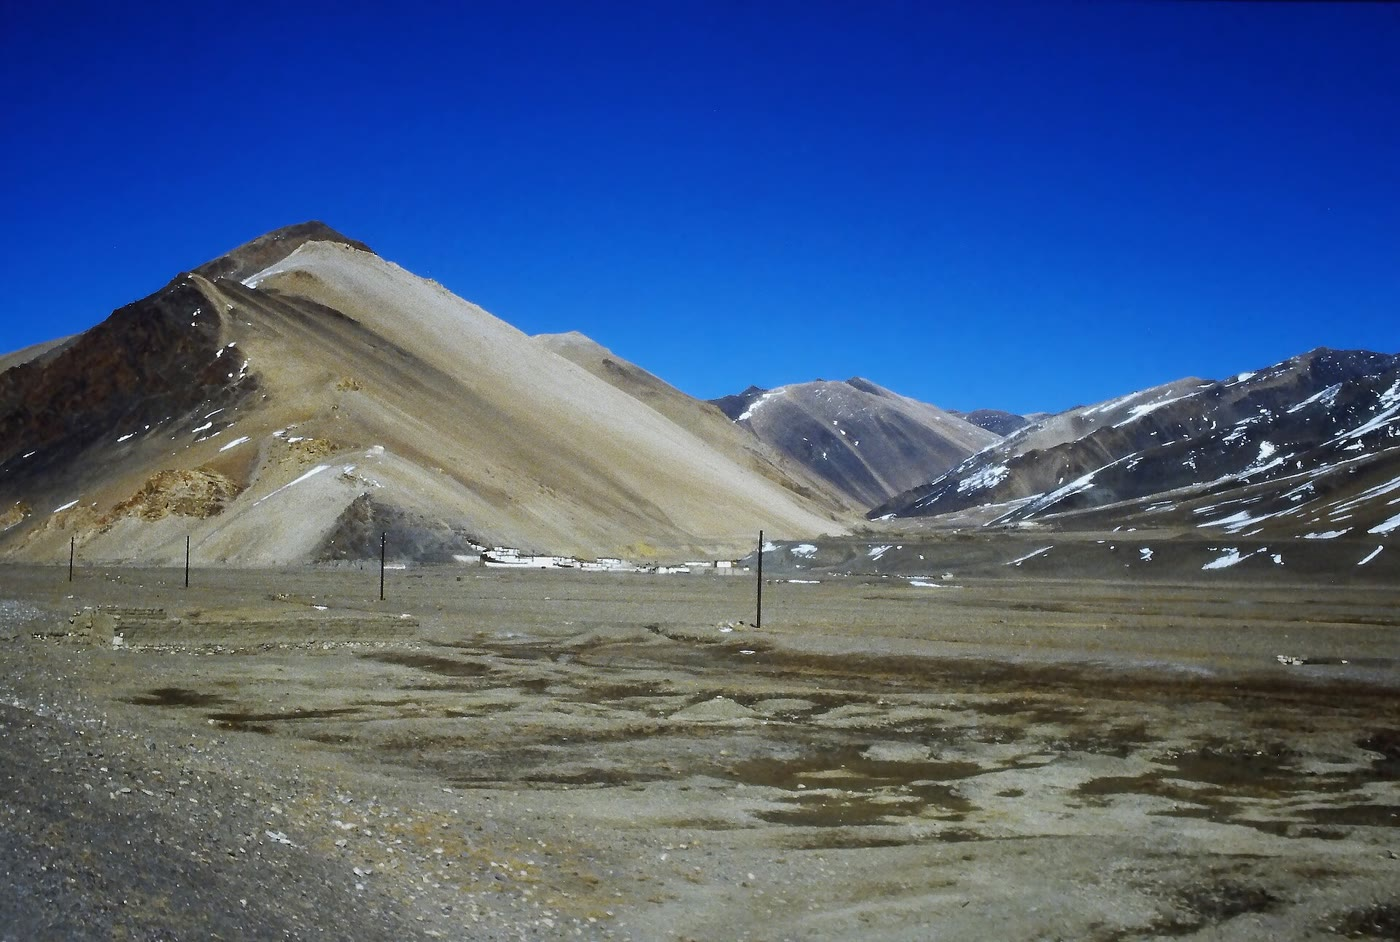
\includegraphics[width=0.66\linewidth]{images/book4/b2-14-tibet-plateau.jpg}
\par\smallskip{\small La meseta del Tíbet entre Nepal y Shigatse: un fondo plano de grava y
pastos escasos, con una aldea, entre montañas desnudas cubiertas de canchales, todo ello a más de
cuatro kilómetros sobre el nivel del mar.
Fotografía de Jan Kranendonk, 1987, CC BY-SA 4.0.}
\end{omfigure}
% ledger: data:b4-etopo-tibet

\subsection{El peso de una meseta}

Una meseta pesa sobre su entorno. A cualquier profundidad hasta la base de su raíz, una columna
bajo la meseta está sometida a una presión mayor que una columna bajo las tierras bajas vecinas;
solo en la profundidad de compensación son iguales. La columna alta empuja hacia fuera.

\begin{proposition}[Exceso de energía potencial de una meseta]\label{prop:b2:himalaya-andes:gpe}
Con las hipótesis de la \cref{prop:b2:himalaya-andes:airy}, con una gravedad $g$, la integral del
exceso de presión litostática de la columna de la meseta sobre la columna normal, desde la cima
de la meseta hasta la profundidad de compensación en la base de su raíz $r$, es
\[
  \Delta F = \rho_c g h \left(H + \frac{h}{2} + \frac{r}{2}\right) .
\]
Es el exceso de energía potencial gravitatoria de la columna de la meseta por unidad de área, y la
fuerza por unidad de longitud del borde de la meseta con la que esta empuja sobre su
entorno.
\end{proposition}

\begin{proof}
Mídase la profundidad $z$ hacia abajo desde el nivel del mar. En la columna de la meseta la presión es $p_1 =
\rho_c g (z + h)$ de $z = -h$ a $L = H + r$. En la columna normal es nula por encima del nivel
del mar, $\rho_c g z$ en la corteza, y $\rho_c g H + \rho_m g (z - H)$ por debajo. La diferencia $p_1
- p_0$ sube de 0 en $z = -h$ a $\rho_c g h$ al nivel del mar; conserva este valor a través de la
corteza normal, donde ambas columnas son corteza; por debajo de $z = H$ disminuye linealmente, en
$(\rho_m - \rho_c) g$ por metro, y se anula en $L$ ya que $(\rho_m - \rho_c) r = \rho_c
h$. La integral es el área de este trapecio: $\rho_c g h\,(h/2 + H + r/2)$. El trabajo realizado por
las presiones cuando las dos columnas intercambian materia lateralmente es esta integral, y por eso
mide a la vez la energía y el empuje.
\end{proof}

\begin{omfigure}
\centering
% figdata/bachelor-2/plateaus.py part pressure (h = 4.8 km, H = 35 km, 2700 and 3300 kg/m3)
\begin{tikzpicture}
\begin{axis}[width=0.62\linewidth, height=5.6cm, y dir=reverse, xmin=0, xmax=160, ymin=-12,
  ymax=60, xlabel={exceso de presión $p_1 - p_0$ (\unit{MPa})}, ylabel={profundidad bajo el nivel del mar
  (\unit{km})}, tick label style={font=\scriptsize}, label style={font=\small},
  xtick pos=bottom, ytick pos=left, clip=false]
\addplot[fill=omThm!20, draw=omThm, line width=1pt] table[x expr=\thisrow{p_high_MPa}-\thisrow{p_ref_MPa}, y=z_km] {figdata/out/bachelor-2-plateaus-pressure.dat} \closedcycle;
\draw[dashed] (axis cs:0,0) -- (axis cs:160,0);
\draw[dashed] (axis cs:0,35) -- (axis cs:160,35);
\draw[dashed] (axis cs:0,56.6) -- (axis cs:160,56.6);
\node[font=\scriptsize, anchor=north east, align=right] at (axis cs:160,0) {nivel\\del mar};
\node[font=\scriptsize, anchor=north east] at (axis cs:160,35) {Moho normal, $H$};
\node[font=\scriptsize, anchor=south east] at (axis cs:160,56.6) {base de la raíz, $H + r$};
\node[font=\scriptsize, anchor=west] at (axis cs:100,-8.4) {cima de la meseta, $-h$};
\node[font=\scriptsize, align=center] at (axis cs:60,20) {área $= \Delta F$\\$\approx\qty{6.1e12}{N.m^{-1}}$};
\end{axis}
\end{tikzpicture}
\par\smallskip{\small El exceso de presión litostática de una columna de meseta sobre una columna
normal, para $h = \qty{4.8}{km}$, $H = \qty{35}{km}$ y densidades de 2700 y
\qty{3300}{kg.m^{-3}}: sube a través de la meseta, se mantiene en $\rho_c g h = \qty{127}{MPa}$
a través de la corteza normal y cae a cero en la base de la raíz. El área sombreada es el
exceso de energía potencial de la \cref{prop:b2:himalaya-andes:gpe}.}
\end{omfigure}
% values (plateaus.py): tibet_gpe 6.12179e12 N/m for h = 4.8

Para el Tíbet, $r = 4.5 \times 4.8 = \qty{21.6}{km}$ y $\Delta F = 2700 \times 9.8 \times 4800
\times (35000 + 2400 + 10800) \approx \qty{6.1e12}{N.m^{-1}}$. Repartido sobre una litosfera
de \qty{100}{km} de espesor, supone un esfuerzo medio en exceso de unos \qty{60}{MPa}, del orden de los
esfuerzos que rompen las rocas. Una meseta tan pesada ya no puede limitarse a elevarse: tiende a extenderse.

\begin{definition}[Colapso gravitacional]\label{def:b2:himalaya-andes:collapse}
El \emph{colapso gravitacional}\index{colapso gravitacional (de un orógeno)} de un \omterm{def:b2:alpine-orogen:orogen}{orógeno}
es la extensión lateral de su corteza engrosada bajo su propio peso, por extensión de las regiones
altas y flujo o cabalgamiento hacia fuera en los bordes, impulsada por el exceso de energía potencial de
las columnas engrosadas.
\end{definition}

El Tíbet se está estirando mientras la India sigue empujándolo. A través del sur del Tíbet, rifts
norte--sur cortan la meseta y acomodan una extensión este--oeste: unos $9 \pm \qty{2}{mm}$ al año en
total entre \ang{81} y \ang{92}~E, $1.3 \pm \qty{0.3}{mm}$ al año solo en el rift de
Yadong--Gulu; al norte de Nepal, las estaciones GPS muestran que el sur de la meseta se estira unos
\num{12e-9} al año. Los terremotos cuentan la misma historia: las fallas inversas y el \omterm{def:b2:himalaya-andes:thickening}{engrosamiento cortical}
dominan en las tierras más bajas que rodean la meseta, y las fallas de desgarre y normales, en su interior.
Por qué se extiende es objeto de debate. En el este de la meseta la extensión se ha interpretado como \omterm{def:b2:himalaya-andes:collapse}{colapso
gravitacional} impulsado por el peso de la meseta; en el sur, otros la relacionan con la forma curva
del arco himalayo, a lo largo del cual divergen los cabalgamientos, o con el deslizamiento de la India por debajo.
% ledger: wang21:rifts, ader12:extension

\subsection{Escapar lateralmente}

\begin{definition}[Extrusión lateral]\label{def:b2:himalaya-andes:extrusion}
La \emph{extrusión lateral}\index{extrusión lateral} (tectónica de escape) es la expulsión lateral de
bloques de corteza o de litosfera desde una zona de colisión, a lo largo de grandes fallas de desgarre,
aproximadamente perpendicular a la dirección de convergencia, hacia un borde libre.
\end{definition}

Al este del Tíbet, Asia no solo se acorta; también es empujada a un lado. Largas fallas de desgarre
sinistrales, entre ellas las del río Rojo y del Altyn Tagh, se interpretan como guías del
escape hacia el este y el sureste de grandes bloques, primero el bloque de Sonda del Sudeste Asiático,
después el Tíbet y el sur de China, mientras se abrían rifts y jóvenes cuencas oceánicas en sus extremos.
Experimentos en los que se empujaba un punzón rígido contra una capa de plastilina produjeron fallas de este tipo;
los modelos que trataban Asia como una lámina viscosa continua produjeron en cambio un engrosamiento extenso, sin
grandes fallas. El GPS respalda el movimiento de bloques: respecto de la Siberia estable, la cuenca del
Tarim se mueve aproximadamente hacia el norte a unos \qty{14}{mm} al año y el sur de China hacia el este-sureste
a unos \qty{8}{mm} al año. Cuánto del avance de la India se ha absorbido por engrosamiento y cuánto
por extrusión sigue siendo objeto de discusión.
% ledger: jiao23:extrusion

\section{Los Andes}\label{sec:b2:himalaya-andes:andes}

La placa de Nazca se hunde bajo Sudamérica a unos \qty{72}{mm} al año cerca de
\ang{20}~S, hacia el este-nordeste, según las velocidades angulares de NNR-MORVEL56. No ha llegado
ningún continente, y sin embargo los Andes Centrales sostienen la segunda meseta más alta de la Tierra.
% ledger: nnr56:poles
% values (plateaus.py): v_nazca_southamerica 72.52 mm/yr, azimuth 74.5

De oeste a este, entre unos \ang{15} y \ang{27}~S, comprenden cinco zonas: el
\emph{antearco}; la \emph{Cordillera Occidental}, el arco volcánico; la alta meseta, el
\emph{Altiplano} al norte y la \emph{Puna} al sur; la \emph{Cordillera
Oriental}; y el \omterm{def:b2:alpine-orogen:ftb}{cinturón de pliegues y cabalgamientos} de piel fina de la \emph{zona subandina}, que
pasa a la llanura del Chaco. El perfil anterior las atraviesa a \ang{20}~S: desde la fosa,
cuyo nodo más profundo está a \qty{7.7}{km} bajo el nivel del mar a \ang{71.4}~W, la superficie sube
más de \qty{11}{km} en unos \qty{240}{km} hasta el borde de la meseta a \ang{69.1}~W;
la meseta se mantiene por encima de \qty{3000}{m} a lo largo de \qty{440}{km} con una
media de \qty{3760}{m}. La altura media es de \qty{3.7}{km} en el Altiplano y de \qty{4.4}{km} en
la Puna. Al norte de \ang{23}~S el Moho está en general a más de \qty{60}{km}; bajo el
Altiplano central la corteza tiene de 59 a \qty{64}{km} de espesor.
% ledger: gerbault05:andes, gerbault05:moho, data:b4-etopo-andes

\begin{omfigure}
\centering
\begin{tikzpicture}[x=0.56cm, y=0.38cm, font=\scriptsize]
% mantle background
\fill[gray!12] (0,-2.6) -- (5,-3.6) -- (8,-5.6) -- (10,-9.1) -- (12,-12.6) -- (13.2,-14.6) -- (26,-14.6)
  -- (26,-4.5) -- (20,-4.7) -- (17.5,-6.0) -- (15,-7.3) -- (11,-7.0) -- (9.5,-6.2) -- (8,-4) -- (5,-2)
  -- (0,-1) -- cycle;
% ocean water
\fill[blue!8] (0,0) -- (6.33,0) -- (5,-2) -- (0,-1) -- cycle;
% Nazca slab
\fill[gray!45] (0,-1) -- (5,-2) -- (8,-4) -- (10,-7.5) -- (12,-11) -- (14,-14.5) -- (13.2,-14.6)
  -- (12,-12.6) -- (10,-9.1) -- (8,-5.6) -- (5,-3.6) -- (0,-2.6) -- cycle;
% South American crust
\fill[orange!22] (5,-2) -- (8,1) -- (9,1.9) -- (10.2,2.0) -- (11,2.0) -- (15,2.0) -- (15.6,2.6) -- (16.8,2.4)
  -- (17.5,1.6) -- (20,0.6) -- (20.6,0.4) -- (26,0.3) -- (26,-4.5) -- (20,-4.7) -- (17.5,-6.0) -- (15,-7.3)
  -- (11,-7.0) -- (9.5,-6.2) -- (8,-4) -- cycle;
% Altiplano basin fill
\fill[yellow!45] (11,2.0) -- (15,2.0) -- (14.6,1.0) -- (11.4,1.0) -- cycle;
% surface line
\draw[line width=0.5pt] (0,-1) -- (5,-2) -- (8,1) -- (9,1.9) -- (10.2,2.0) -- (11,2.0) -- (15,2.0) -- (15.6,2.6)
  -- (16.8,2.4) -- (17.5,1.6) -- (20,0.6) -- (20.6,0.4) -- (26,0.3);
% arc volcanoes
\fill[red!60!black] (8.8,1.75) -- (9.2,2.9) -- (9.6,1.95) -- cycle;
\fill[red!60!black] (9.8,1.95) -- (10.2,2.8) -- (10.6,2.0) -- cycle;
\draw[red!60!black, decorate, decoration={snake, amplitude=0.6pt, segment length=4pt}] (10.8,-8.0) -- (9.9,1.6);
% Subandean decollement and splays
\draw[thick] (16.0,-1.2) -- (20.55,0.42);
\draw (17.4,-0.7) -- (17.85,1.45);
\draw (18.4,-0.35) -- (18.8,1.08);
\draw (19.4,0.0) -- (19.7,0.72);
% Moho
\draw[dashed] (8,-4) -- (9.5,-6.2) -- (11,-7.0) -- (15,-7.3) -- (17.5,-6.0) -- (20,-4.7) -- (26,-4.5);
% labels
\node at (2.6,-0.5) {Pacífico};
\node at (2.4,-2.2) {placa de Nazca};
\draw[-{Latex[length=1.6mm]}] (1.6,-2.8) -- (3.2,-3.0);
\node[anchor=south] (tr) at (4.3,0.9) {fosa};
\draw[->] (tr.south) -- (5,-1.8);
\node[anchor=south east] at (7.6,1.0) {antearco};
\node[anchor=south, align=center] at (9.7,3.0) {Cordillera\\Occidental (arco)};
\node[anchor=south] at (13,2.1) {Altiplano};
\node[anchor=south, align=center] at (16.4,2.7) {Cordillera\\Oriental};
\node[anchor=south west] at (18.6,1.3) {Subandino};
\node[anchor=south] at (23.5,0.4) {llanura del Chaco};
\node at (13,-3.2) {corteza gruesa};
\node at (23.2,-2.0) {escudo brasileño};
\node[anchor=north] at (23.2,-4.6) {Moho};
\node at (14.2,-9.6) {cuña de manto};
\node at (21,-10) {manto};
\node[rotate=-50] at (12.75,-12.9) {placa};
\draw[-{Latex[length=2mm]}] (1.2,4.6) -- (0.2,4.6);
\node[anchor=south] at (0.7,4.6) {O};
\draw[-{Latex[length=2mm]}] (24.8,4.6) -- (25.8,4.6);
\node[anchor=south] at (25.3,4.6) {E};
\end{tikzpicture}
\par\smallskip{\small Corte esquemático a través de los Andes Centrales cerca de \ang{20}~S (sin
escala). La placa de Nazca se hunde bajo el antearco; el \omterm{def:b2:magma-emplacement:magma}{magma} sube desde la cuña de manto (línea
ondulada) hasta el arco de la Cordillera Occidental; el Altiplano, con su grueso relleno de cuenca, se sitúa
entre las dos cordilleras, sobre una corteza de unos \qty{60}{km} de espesor; el cinturón subandino
de piel fina cabalga hacia el este sobre el escudo brasileño.}
\end{omfigure}
% ledger: gerbault05:andes, gerbault05:moho

\subsection{Cómo se engrosó la corteza}

¿De dónde vino la corteza adicional del Altiplano? El primer candidato es el acortamiento:
si se comprime una franja de corteza, se engruesa conservando el área de su sección.

\begin{proposition}[Engrosamiento por acortamiento]\label{prop:b2:himalaya-andes:shortening}
Sea una corteza de espesor uniforme $H$ acortada, sin ganancia ni pérdida de roca, hasta una corteza
de espesor $T$ en una anchura $W$, con la sección paralela al acortamiento. Su
anchura original era $W_0 = W T/H$, y el acortamiento es
\[
  S = W_0 - W = W\,\frac{T - H}{H} .
\]
\end{proposition}

\begin{proof}
El área de la sección de la corteza se conserva, como en la compensación de áreas de la
\cref{prop:b2:alpine-orogen:balance}: $W_0 H = W T$. Por tanto $W_0 = WT/H$ y $S = W_0 - W =
W(T - H)/H$.
\end{proof}

A \ang{20}~S la meseta tiene unos \qty{440}{km} de anchura; si su corteza, de unos \qty{60}{km} de espesor,
tuvo en su día \qty{35}{km}, el acortamiento necesario es $440 \times 25/35 \approx \qty{314}{km}$.
Los \omterm{def:b2:alpine-orogen:balanced}{cortes compensados} cerca de 16--\ang{21}~S hallan unos \qty{50}{km} de acortamiento en el Altiplano
y más de \qty{200}{km} en la zona subandina desde el Oligoceno. Los volúmenes corticales
calculados a partir del acortamiento quedan cerca de un \qty{20}{\percent} por debajo de los calculados a partir de la profundidad
del Moho. Parte de la diferencia puede deberse a hipótesis erróneas, sobre el espesor inicial o
la naturaleza del Moho sísmico; parte puede ser corteza añadida por otras vías. Una compilación cerca de
\ang{21}~S atribuye al acortamiento tectónico al menos un \qty{55}{\percent} de la raíz, a la
hidratación de la cuña de manto del antearco hasta un \qty{20}{\percent}, y al aporte magmático y a la
erosión tectónica solo cerca de un \qty{5}{\percent}. La roca también puede desplazarse dentro de la cordillera:
las diferencias de espesor cortical crean diferencias de energía potencial, como en el Tíbet, y
estas pueden impulsar el flujo de la corteza inferior caliente de las zonas gruesas a las delgadas.
% ledger: gerbault05:andes, gerbault05:volume, gerbault05:moho, data:b4-etopo-andes

\begin{omfigure}
\centering
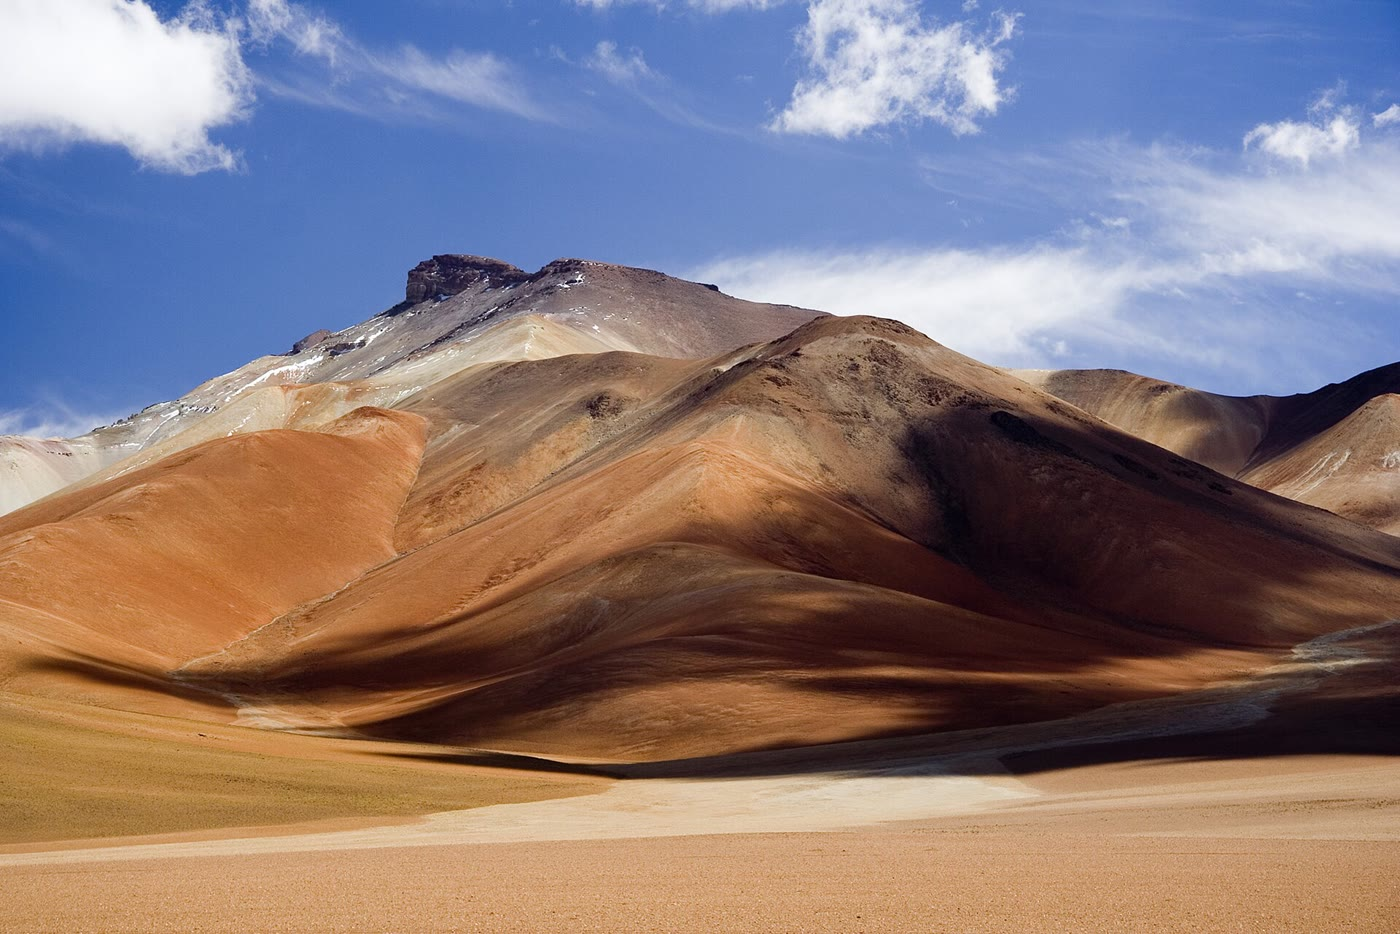
\includegraphics[width=0.66\linewidth]{images/book4/b2-14-altiplano.jpg}
\par\smallskip{\small El Altiplano boliviano: una llanura de arena y grava al pie de
colinas desnudas teñidas de rojo, ocre y gris por sus rocas. Fotografía de Luca Galuzzi, 2006, CC BY-SA 2.5.}
\end{omfigure}
% ledger: gerbault05:andes

\subsection{Placas planas y raíces perdidas}

El ángulo de la placa que subduce no es fijo, y eso importa en superficie.

\begin{definition}[Subducción plana]\label{def:b2:himalaya-andes:flat-slab}
La \emph{subducción plana}\index{subducción plana} es una subducción en la que la placa que subduce,
tras su primer descenso, discurre casi horizontal bajo la placa cabalgante a lo largo de cientos
de kilómetros antes de volver a hundirse.
\end{definition}

A lo largo de los Andes, dos segmentos de la placa de Nazca son hoy planos: el segmento peruano, plano
desde hace unos \qty{15}{Ma}, y el segmento pampeano, desde hace unos \qty{18}{Ma}. Sobre ellos no
hay volcanes activos. Cuando la placa pampeana se aplanó, el arco se desplazó hacia el interior y emitió
menos lava; sobre los segmentos planos ha enmudecido. El espacio arco--fosa del volumen de primer año
explica el desplazamiento hacia el interior: cuanto más suave es la placa bajo el arco, más lejos de la fosa
alcanza la profundidad a la que funde la cuña; y una placa que se mantiene plana por encima de esa profundidad no deja
ninguna cuña de manto caliente que pueda fundir.
% ledger: gauthier24:flat

\begin{definition}[Delaminación litosférica]\label{def:b2:himalaya-andes:delamination}
La \emph{delaminación litosférica}\index{delaminación litosférica} es el desprendimiento y el
hundimiento en la astenosfera de la parte inferior de una litosfera engrosada, su manto
litosférico y a veces una corteza inferior densa, sustituida por astenosfera caliente.
\end{definition}

Se ha propuesto una delaminación bajo el sur de la Puna, entre \ang{24} y \ang{27}~S,
hace unos 2 a \qty{3}{Ma}, donde hicieron erupción lavas máficas jóvenes; y a lo largo de la meseta, los cambios
de espesor cortical y de altitud se han relacionado con un manto litosférico ya eliminado
bajo el sur del Altiplano y todavía no del todo bajo el Altiplano central. Perder una
tapa de manto densa aligera la columna restante: la superficie se eleva sin más
acortamiento. La Puna está cerca de \qty{1}{km} más alta que el Altiplano sobre una corteza unos
\qty{11}{km} más delgada, un contraste que requiere o bien una corteza más ligera en la Puna o bien un manto más ligero
bajo ella.
% ledger: gerbault05:delamination, gerbault05:moho

\section{Dos cordilleras comparadas}\label{sec:b2:himalaya-andes:compared}

Las dos mesetas se parecen vistas de lejos y difieren en casi todo lo demás, como reúne la tabla
siguiente.

\begin{omfigure}
\centering\small
\begin{tabular}{>{\raggedright\arraybackslash}p{0.2\linewidth}|>{\raggedright\arraybackslash}p{0.34\linewidth}|>{\raggedright\arraybackslash}p{0.34\linewidth}}
 & Himalaya y Tíbet & Andes Centrales \\ \hline
motor & continente contra continente tras el cierre del océano & placa oceánica que se hunde bajo un continente \\
eje & sutura con \omterm{def:b2:alpine-orogen:ophiolite}{ofiolitas} & arco volcánico sobre la placa que subduce \\
magmatismo & fundidos corticales: \omterm{def:b2:crustal-melting:leucogranite}{leucogranitos} & andesitas de arco; lavas máficas donde se perdió la litosfera \\
convergencia & unos \qty{45}{mm} al año, la mitad absorbida en la cordillera & unos \qty{72}{mm} al año, consumidos sobre todo por la subducción \\
grandes terremotos & en el MHT, Assam 1950, $M_w \approx 8.5$ & en la interfaz de subducción, Chile 1960, $M_w$ 9.5 \\
meseta & media \qty{4.8}{km} sobre \qty{1180}{km}; corteza de 70--\qty{75}{km} & media \qty{3.8}{km} sobre \qty{440}{km}; corteza de unos \qty{60}{km} \\
tectónica de la meseta & extensión este--oeste, extrusión & acortamiento en los flancos; delaminación propuesta \\
antepaís & antefosa indogangética y \omterm{def:b2:alpine-orogen:foreland}{molasa} de los Siwalik & cinturón subandino y llanura del Chaco \\
\end{tabular}
\par\smallskip{\small Las dos cordilleras una junto a otra; las fuentes se citan en las secciones anteriores,
y el terremoto de Chile es el mayor registrado desde 1900.}
\end{omfigure}
% ledger: lave00:setting, lave00:siwaliks, weinberg16:himalaya, ader12:mht, ader12:quakes, usgs:largest, gerbault05:andes, gerbault05:moho, gerbault05:delamination, nnr56:poles, data:b4-etopo-tibet, data:b4-etopo-andes, cattin01:crust, wang21:rifts, jiao23:extrusion

La diferencia más profunda está en lo que se hunde. En los Andes la placa oceánica sigue hundiéndose, y
la mayor parte de la convergencia, unos \qty{72}{mm} al año, se consume en la fosa; acortar la
placa superior \qty{310}{km} en unos 30 millones de años solo requeriría unos \qty{10}{mm} al
año. En el Himalaya nada ligero puede hundirse por mucho tiempo, de modo que la convergencia se gasta en
apilar, engrosar y apartar Asia. Ambas cordilleras desarrollan mesetas porque una corteza gruesa
es una corteza alta; ambas mesetas dejan de elevarse cuando su propio peso equilibra el empuje en sus
bordes, y entonces se extienden.
% ledger: nnr56:poles, gerbault05:andes, ader12:mht, jiao23:extrusion

\section{¿Qué altura puede tener una montaña?}\label{sec:b2:himalaya-andes:heights}

La cumbre más alta, el Everest, se alza \qty{8848.86}{m} sobre el nivel del mar según la medición conjunta
anunciada en 2020. ¿Por qué no veinte kilómetros? Una cota aproximada procede de la resistencia de la roca.

\begin{proposition}[Un límite de altura impuesto por la resistencia de la roca]\label{prop:b2:himalaya-andes:height}
Una columna de roca de densidad $\rho$ que se alza una altura $h$ sobre su entorno, sin
apoyo lateral por encima del nivel de este, soporta en su pie un esfuerzo vertical $\rho g h$ y un
esfuerzo horizontal nulo en sus caras libres, y por tanto un esfuerzo diferencial $\rho g h$. Si la
roca rompe al esfuerzo diferencial $\sigma_d$, la columna solo se sostiene si $h < \sigma_d/(\rho
g)$.
\end{proposition}

\begin{proof}
En el pie de la columna el esfuerzo vertical es el peso de la roca suprayacente por unidad de área,
$\rho g h$. Las caras son libres, de modo que allí el esfuerzo horizontal es nulo. El esfuerzo diferencial
es la diferencia entre los esfuerzos principales mayor y menor, aquí $\rho g h - 0$.
La rotura solo se evita si se mantiene por debajo de $\sigma_d$.
\end{proof}

Una montaña real tiene flancos inclinados que contienen su núcleo, de modo que el esfuerzo bajo ella es
menor; como orden de magnitud, tómese la mitad, $\rho g h/2$. Para el Everest, $2700 \times 9.8
\times 8849/2 \approx \qty{117}{MPa}$. La ley de Byerlee del volumen de primer año sitúa la resistencia
friccional de la roca en una falla bajo un esfuerzo normal de \qty{200}{MPa} en $50 + 0.6 \times 200 =
\qty{170}{MPa}$: el mismo orden. Una montaña tres veces más alta cargaría su base muy por encima de
lo que la roca puede soportar; rompería y se extendería. En la Tierra, las cumbres de ocho a nueve kilómetros
están cerca del límite, y una meseta, que se extiende mucho antes de que rompan sus cumbres, se estabiliza
en cinco.
% ledger: tht:everest, byerlee:1975

\section*{Ejercicios}\label{sec:b2:himalaya-andes:exercises}

Datos para los ejercicios: $g = \qty{9.8}{m.s^{-2}}$; densidades de la corteza y del manto
\qty{2700}{kg.m^{-3}} y \qty{3300}{kg.m^{-3}} salvo indicación contraria; corteza normal $H =
\qty{35}{km}$.

\begin{exercise}[$\star$]\label{exo:b2:himalaya-andes:1}
Una meseta se encuentra a una altitud media de \qty{3.0}{km}. Con ayuda de la
\cref{prop:b2:himalaya-andes:airy}, calcúlense (a) su raíz de Airy, (b) su espesor cortical.
(c) ¿Cuánto la elevarían \qty{10}{km} más de corteza?
\end{exercise}

\begin{exercise}[$\star$]\label{exo:b2:himalaya-andes:2}
Un recorrido por el Himalaya de Nepal va de la llanura del Ganges a la meseta del Tíbet.
(a) Enumérense, por orden, las unidades que atraviesa y las fallas que las separan. (b) ¿Qué falla
es una falla normal? (c) ¿Cómo cambia el grado metamórfico hacia el norte hasta la secuencia del Alto
Himalaya, y después por encima de ella?
\end{exercise}

\begin{exercise}[$\star$]\label{exo:b2:himalaya-andes:3}
En el centro de Nepal, una terraza fluvial abandonada hace \qty{9.2}{kyr} se ha acortado
\qty{196.5}{m} a través de los pliegues del Cabalgamiento Frontal Principal. (a) Calcúlese la velocidad media de
acortamiento en milímetros al año. (b) Compárese con la convergencia GPS a través de la cordillera,
\qty{17.8}{mm} al año. (c) ¿Qué dice esta coincidencia sobre las fallas situadas al norte del MFT?
\end{exercise}

\begin{exercise}[$\star$]\label{exo:b2:himalaya-andes:4}
Clasifíquese cada observación como propia de un \omterm{def:b2:himalaya-andes:types}{orógeno de colisión}, de un \omterm{def:b2:himalaya-andes:types}{orógeno de tipo andino} o de ambos: (a) una sutura jalonada
de \omterm{def:b2:alpine-orogen:ophiolite}{ofiolitas}; (b) una línea de volcanes andesíticos activos; (c) \omterm{def:b2:crustal-melting:leucogranite}{leucogranitos} procedentes de la fusión de la
corteza; (d) una fosa oceánica profunda a lo largo del frente; (e) una \omterm{def:b2:alpine-orogen:foreland}{cuenca de antepaís} con \omterm{def:b2:alpine-orogen:foreland}{molasa};
(f) grandes terremotos en una falla de buzamiento suave bajo la cordillera.
\end{exercise}

\begin{exercise}[$\star\star$]\label{exo:b2:himalaya-andes:5}
La India se mueve a \qty{45}{mm} al año respecto de Eurasia a través del Himalaya; a través de Nepal, la
propia cordillera absorbe \qty{17.8}{mm} al año en el este y \qty{20.5}{mm} al año en el oeste.
(a) ¿Qué fracción de la convergencia absorbe la cordillera en cada caso? (b) ¿Adónde va el
resto? (c) En \qty{10}{Myr}, ¿cuánto acortamiento representa el resto?
\end{exercise}

\begin{exercise}[$\star\star$]\label{exo:b2:himalaya-andes:6}
(a) Con ayuda de la \cref{prop:b2:himalaya-andes:gpe}, calcúlese el exceso de energía potencial del
Altiplano, de altitud media \qty{3.7}{km}. (b) Compárese con el del Tíbet a \qty{4.8}{km}.
(c) Demuéstrese que para una meseta baja, $h \ll H$, $\Delta F$ crece proporcionalmente a $h$, y para una
alta, más deprisa: ¿qué implica eso para el crecimiento de una meseta?
\end{exercise}

\begin{exercise}[$\star\star$]\label{exo:b2:himalaya-andes:7}
(a) Calcúlese $\rho g h/2$ bajo el Everest, de \qty{8848.86}{m} de altura, con $\rho =
\qty{2700}{kg.m^{-3}}$. (b) Según la ley de Byerlee, $\tau = 0.85\,\sigma_n$ por debajo de \qty{200}{MPa} de
esfuerzo normal y $\tau = \qty{50}{MPa} + 0.6\,\sigma_n$ por encima; calcúlese $\tau$ para $\sigma_n =
100$ y \qty{200}{MPa}. (c) ¿Qué altura permitiría una resistencia de \qty{170}{MPa}, con la misma
regla de orden de magnitud?
\end{exercise}

\begin{exercise}[$\star\star$]\label{exo:b2:himalaya-andes:8}
Los rifts del sur del Tíbet absorben $9 \pm \qty{2}{mm}$ al año de extensión este--oeste entre
\ang{81} y \ang{92}~E. (a) ¿Qué anchura tiene ese tramo a \ang{30}~N, con \qty{111.19}{km} por
grado sobre un meridiano? (b) Calcúlese la velocidad media de deformación extensional, por año y por segundo,
con su intervalo. (c) Compárese con el $(12.4 \pm 4.7) \times 10^{-9}$ al año hallado por GPS al norte de Nepal.
\end{exercise}

\begin{exercise}[$\star\star$]\label{exo:b2:himalaya-andes:9}
El Cabalgamiento Principal del Himalaya, bloqueado bajo Nepal, acumula un déficit de momento de
\qty{6.6e19}{N.m} al año; los terremotos de los últimos 500 años solo liberaron
\qty{0.9e19}{N.m} al año. (a) ¿Qué fracción del déficit liberaron? (b) Con $M_0 =
10^{1.5 M_w + 9.1}$\,\unit{N.m}, calcúlese el momento de un terremoto de $M_w$ 8.5. (c) ¿Con qué frecuencia
harían falta terremotos así para equilibrar el déficit?
\end{exercise}

\begin{exercise}[$\star\star\star$]\label{exo:b2:himalaya-andes:10}
La Puna está \qty{0.7}{km} más alta que el Altiplano (4.4 frente a \qty{3.7}{km}) sobre una corteza
\qty{11}{km} más delgada. Tómese la corteza del Altiplano de \qty{61.5}{km} de espesor y de densidad
\qty{2800}{kg.m^{-3}}, y un manto de \qty{3300}{kg.m^{-3}} bajo ambas. (a) Escríbase la
igualdad de las masas de las dos columnas por encima de una profundidad de compensación común. (b) Hállese la
densidad que debe tener la corteza de la Puna si solo la corteza compensa la diferencia. (c) Compárese
con los 150 a \qty{200}{kg.m^{-3}} citados, y dígase qué más podría explicar el contraste.
\end{exercise}

\begin{exercise}[$\star\star\star$]\label{exo:b2:himalaya-andes:11}
El frente volcánico se sitúa donde el techo de la placa que subduce está a \qty{105}{km} de profundidad. (a) Para una placa
que buza uniformemente \ang{30}, calcúlese el espacio arco--fosa con la fórmula del volumen de primer
año. (b) La placa buza ahora \ang{30} hasta \qty{90}{km} y después solo \ang{4}: calcúlense
el nuevo espacio y el desplazamiento del arco hacia el interior. (c) ¿Qué le ocurre al arco si la placa se aplana
a \qty{95}{km} de profundidad y se mantiene así a lo largo de \qty{300}{km}?
\end{exercise}

\begin{exercise}[$\star\star\star$]\label{exo:b2:himalaya-andes:12}
La erosión elimina unos \qty{300}{km^3} de roca por kilómetro de Himalaya y por millón de años.
La India aporta corteza de \qty{37.5}{km} de espesor a \qty{21}{mm} al año. (a) ¿Cuánta corteza por
kilómetro de cordillera y por millón de años entra en la cordillera? (b) ¿Qué fracción elimina la erosión?
(c) ¿Dónde puede estar el resto?
\end{exercise}

\begin{problem}[{Problema de fin de semana --- dos mesetas}]\label{pb:b2:himalaya-andes:1}
Los perfiles en franja de este capítulo dan la altitud media de los nodos a través del Tíbet
(\qtyrange{86}{90}{\degree} E) y a través de los Andes Centrales (\qtyrange{19}{21}{\degree} S).
Muestreados cada \ang{1.5} de latitud y cada grado de longitud, y redondeados a \qty{10}{m},
dan lo siguiente. Salvo indicación contraria, $g = \qty{9.8}{m.s^{-2}}$, $\rho_c = \qty{2700}{kg.m^{-3}}$,
$\rho_m = \qty{3300}{kg.m^{-3}}$ y la corteza normal tiene $H = \qty{35}{km}$ de espesor.

\smallskip
\begin{center}\small
\begin{tabular}{l|ccccccccc}
latitud (\unit{\degree} N) & 26.5 & 28.0 & 29.5 & 31.0 & 32.5 & 34.0 & 35.5 & 37.0 & 38.5 \\ \hline
altitud media (\unit{m}) & 70 & 5000 & 5030 & 4830 & 5020 & 5150 & 5050 & 4470 & 2210
\end{tabular}

\smallskip
\begin{tabular}{l|cccccccc}
longitud (\unit{\degree}) & $-71$ & $-70$ & $-69$ & $-68$ & $-67$ & $-66$ & $-65$ & $-64$ \\ \hline
altitud media (\unit{m}) & $-3310$ & 970 & 4150 & 3720 & 3740 & 4010 & 3030 & 1170
\end{tabular}
\end{center}
\smallskip

\noindent\textbf{Parte I --- Leer los perfiles.}
\begin{enumerate}
\item Tomando como meseta las muestras por encima de \qty{3000}{m}, calcúlese la altitud media del Tíbet
$h_T$, redondeada a \qty{0.1}{km}.
\item Hágase lo mismo para el Altiplano, $h_A$, y compárese con la altura media de
\qty{3.7}{km} citada para el Altiplano y de \qty{4.4}{km} para la Puna.
\item ¿Qué anchura mínima tiene cada meseta según las muestras (\qty{111.19}{km} por
grado de latitud; \qty{104.5}{km} por grado de longitud a \ang{20}~S)?
\item Calcúlese la pendiente media del frente himalayo entre \ang{26.5} y \ang{28.0}~N, en
porcentaje.
\item ¿Por qué el perfil andino es mucho más asimétrico que el tibetano?
\end{enumerate}

\noindent\textbf{Parte II --- Espesores de Airy.}
\begin{enumerate}[resume]
\item Calcúlense la raíz de Airy y el espesor cortical $T_T$ del Tíbet a partir de $h_T$.
\item Hágase lo mismo para el Altiplano, $T_A$.
\item Compárese con los espesores sísmicos, de 70 a \qty{75}{km} bajo el Tíbet y de 59 a
\qty{64}{km} bajo el Altiplano central. ¿Qué estimación se aleja más?
\item ¿Qué densidad cortical haría que el espesor de Airy del Tíbet fuera de \qty{72.5}{km}?
\item ¿Qué densidad daría \qty{61.5}{km} para el Altiplano?
\item Dense dos razones, además de la densidad cortical, por las que un cálculo de Airy local puede
no reproducir la raíz observada.
\item La corteza tiene \qty{37.5}{km} de espesor bajo la India y \qty{72.5}{km} bajo el Tíbet. Con un
contraste de densidad en el Moho de \qty{370}{kg.m^{-3}}, estímese con la placa de Bouguer, $\Delta g
= 2\pi G\,\Delta\rho\,t$, la anomalía de Bouguer de la raíz del Tíbet respecto de la India, siendo $t$ el
espesor adicional bajo el nivel del mar ($G = \qty{6.674e-11}{m^3.kg^{-1}.s^{-2}}$). Compárese con la
diferencia observada de \qty{460}{mGal}.
\end{enumerate}

\noindent\textbf{Parte III --- Acortar el Altiplano.} A \ang{20}~S la meseta tiene
\qty{440}{km} de anchura y su corteza unos \qty{60}{km} de espesor.
\begin{enumerate}[resume]
\item Con ayuda de la \cref{prop:b2:himalaya-andes:shortening}, calcúlense la anchura restituida y el
acortamiento necesario si la corteza tenía antes \qty{35}{km} de espesor.
\item Los \omterm{def:b2:alpine-orogen:balanced}{cortes compensados} dan unos \qty{50}{km} de acortamiento en el Altiplano y
\qty{200}{km} en la zona subandina. ¿Qué fracción del acortamiento necesario falta?
\item Si el acortamiento solo produjo un \qty{55}{\percent} de la corteza adicional, ¿cuánto acortamiento hace
falta?
\item El cinturón subandino es de piel fina. ¿Por qué su acortamiento tiene que engrosar igualmente la corteza
en algún lugar?
\item Supóngase que los \qty{314}{km} de la Parte III se acumularon en \qty{30}{Myr}. Calcúlese la velocidad
media, y la fracción de la convergencia actual Nazca--Sudamérica, \qty{72}{mm} al año, que
representa.
\item ¿Adónde va el resto de la convergencia?
\end{enumerate}

\noindent\textbf{Parte IV --- El peso del Tíbet.}
\begin{enumerate}[resume]
\item Con ayuda de la \cref{prop:b2:himalaya-andes:gpe} con $h_T$, calcúlese el exceso de energía potencial
del Tíbet por unidad de área.
\item Calcúlese para el Altiplano con $h_A$, y la razón entre ambos.
\item Repártase el $\Delta F$ del Tíbet sobre una litosfera de \qty{100}{km} de espesor: ¿qué esfuerzo medio
representa?
\item La extensión del sur del Tíbet, \qty{9}{mm} al año a lo largo de \qty{1060}{km}, ¿qué
deformación anual supone?
\item ¿Por qué puede extenderse el Tíbet de este a oeste mientras la India sigue empujándolo hacia el norte?
\item En resumen: dese el espesor cortical del Tíbet calculado a partir de su altitud media, redondeado
al kilómetro, y la fracción de los \qty{72.5}{km} sísmicos que explica.
\end{enumerate}
\end{problem}
